% !TeX TXS-program:compile = txs:///arara
% arara: pdflatex: {shell: yes, synctex: no, interaction: batchmode}
% arara: pdflatex: {shell: yes, synctex: no, interaction: batchmode} if found('log', '(undefined references|Please rerun|Rerun to get)')

\documentclass{article}
\usepackage[english]{babel}
\usepackage[utf8]{inputenc}
\usepackage[T1]{fontenc}
\usepackage{TangramTikz}
%\usepackage[upright]{fourier}
%\usepackage[scaled=0.875]{helvet}
%\renewcommand\ttdefault{lmtt}
%\usepackage{cabin}
\usepackage{amsmath,amssymb}
\usepackage{fontawesome5}
\usepackage{enumitem}
\usepackage{tabularray}
\usepackage{multicol}
\usepackage{fancyvrb}
\usepackage{fancyhdr}
\fancyhf{}
\renewcommand{\headrulewidth}{0pt}
\lfoot{\sffamily\small [TangramTikz]}
\cfoot{\sffamily\small - \thepage{} -}
\rfoot{\hyperlink{matoc}{\small\faArrowAltCircleUp[regular]}}

%\usepackage{hvlogos}
\usepackage{hologo}
\usepackage{xspace}
\providecommand\tikzlogo{Ti\textit{k}Z}
\providecommand\TeXLive{\TeX{}Live\xspace}
\providecommand\PSTricks{\textsf{PSTricks}\xspace}
\let\pstricks\PSTricks
\let\TikZ\tikzlogo
\newcommand\TableauDocumentation{%
	\begin{tblr}{width=\linewidth,colspec={X[c]X[c]X[c]X[c]X[c]X[c]},cells={font=\sffamily}}
		{\huge \LaTeX} & & & & &\\
		& {\huge \hologo{pdfLaTeX}} & & & & \\
		& & {\huge \hologo{LuaLaTeX}} & & & \\
		& & & {\huge \TikZ} & & \\
		& & & & {\huge \TeXLive} & \\
		& & & & & {\huge \hologo{MiKTeX}} \\
	\end{tblr}
}

\usepackage{hyperref}
\urlstyle{same}
\hypersetup{pdfborder=0 0 0}
\usepackage[margin=1.5cm]{geometry}
\setlength{\parindent}{0pt}
\definecolor{LightGray}{gray}{0.9}

\def\TPversion{0.1.1}
\def\TPdate{26/01/2023}

\usepackage[most]{tcolorbox}
\tcbuselibrary{minted}
\NewTCBListing{PresentationCode}{ O{blue} m }{%
	sharp corners=downhill,enhanced,arc=12pt,skin=bicolor,%
	colback=#1!1!white,colframe=#1!75!black,colbacklower=white,%
	attach boxed title to top right={yshift=-\tcboxedtitleheight},title=Code \LaTeX,%
	boxed title style={%
		colframe=#1!75!black,colback=#1!15!white,%
		,sharp corners=downhill,arc=12pt,%
	},%
	fonttitle=\color{#1!90!black}\itshape\ttfamily\footnotesize,%
	listing engine=minted,minted style=colorful,
	minted language=tex,minted options={tabsize=4,fontsize=\footnotesize,autogobble},
	#2
}

\newcommand\Cle[1]{{\bfseries\sffamily\textlangle #1\textrangle}}

\begin{document}

\pagestyle{fancy}

\thispagestyle{empty}

\vspace{2cm}

\begin{center}
	\begin{minipage}{0.75\linewidth}
	\begin{tcolorbox}[colframe=yellow,colback=yellow!15]
		\begin{center}
			\begin{tabular}{c}
				{\Huge \texttt{TangramTikz [en]}}\\
				\\
				{\LARGE Tangrams, with Ti\textit{k}Z}, \\
				\\
				{\LARGE with solution and/or color.} \\
			\end{tabular}
			
			\medskip
			
			{\small \texttt{Version \TPversion{} -- \TPdate}}
		\end{center}
	\end{tcolorbox}
\end{minipage}
\end{center}

\vspace{0.5cm}

\begin{center}
	\begin{tabular}{c}
	\texttt{Cédric Pierquet}\\
	{\ttfamily c pierquet -- at -- outlook . fr}\\
	\texttt{\url{https://github.com/cpierquet/TangramTikz}}
\end{tabular}
\end{center}

\vspace{0.5cm}

{$\blacktriangleright$~~Some commands to display existing Tangrams.}

\smallskip

{$\blacktriangleright$~~Create tangram, with postionning manually the pieces.}

\smallskip

{$\blacktriangleright$~~Idea(s) from \url{https://tex.stackexchange.com/questions/407449/typesetting-tangram-figures-in-latex}}

\vspace{1cm}

\begin{center}
	\tikz {\pic[TangPuzz={blue}] at (0,0) {TangBigTri} ;}~~
	\tikz {\pic[TangPuzz={orange}] at (0,0) {TangBigTri} ;}~~
	\tikz {\pic[TangPuzz={purple}] at (0,0) {TangMedTri} ;}~~
	\tikz {\pic[TangPuzz={yellow}] at (0,0) {TangSqua} ;}~~
	\tikz {\pic[TangPuzz={green}] at (0,0) {TangSmalTri} ;}~~
	\tikz {\pic[TangPuzz={cyan}] at (0,0) {TangSmalTri} ;}~~
	\tikz {\pic[TangPuzz={magenta}] at (0,0) {TangPara} ;}~~
	
	\vspace*{1cm}
	
	\TangramTikz[Couleur=orange]<scale=1>{Maison}
	\TangramTikz[Correction]<scale=1>{Maison}
	\TangramTikz[CorrectionCouleur]<scale=1>{Maison}
	\TangramTikz[ListeCouleurs={blue,red,black,orange,purple},CorrectionCouleur]<scale=1>{Maison}
\end{center}

\vspace{0.5cm}

%\hfill{}\textit{Merci aux membres du groupe \faFacebook{} du \og Coin \LaTeX{} \fg{} pour leur aide et leurs idées !}

%\hfill{}\textit{Merci à Denis Bitouzé et à Patrick Bideault pour leurs retours et idées !}

\vfill

\hrule

\medskip

\TableauDocumentation

\medskip

\hrule

\medskip

\newpage

\phantomsection
\hypertarget{matoc}{}

\tableofcontents

\newpage

\part{Introduction}

\section{The package TangramTikz}

\subsection{Source}

Some of the ideas are coming from \url{https://tex.stackexchange.com/questions/407449/typesetting-tangram-figures-in-latex}, specially from Andrew Stacey.

\smallskip

The package has been \textit{built} around the ideas from Andrew Stacey.

\subsection{Loading of the package, used packages}

The package \textsf{TangramTikz} loads into the preamble by :

\begin{PresentationCode}{listing only}
\usepackage{TangramTikz}
\end{PresentationCode}

It's fully copatible with usuals compilations, such as \textsf{latex}, \textsf{pdflatex}, \textsf{lualatex} or \textsf{xelatex}.

\medskip

It loads the packages and libraries :

\begin{itemize}
	\item \texttt{tikz} awith libraries \Cle{calc} ans \Cle{shapes.geometric} ;
	\item \texttt{xstring}, \texttt{xparse}, \texttt{simplekv} and \texttt{listofitems}.
\end{itemize}

\subsection{The package itself}

The idea is to, thanks to \TikZ, propose \textsf{commands} to display a Tangram Puzzle :

\begin{itemize}
	\item with \textit{full} pieces ;
	\item by puzzle with \textit{border} pieces ;
	\item by puzzle with \textit{border colored} pieces.
\end{itemize}

\begin{PresentationCode}{listing only}
%independant command to display a Tangram
\TangramTikz[keys]<options tikz>{tangram_name}
\end{PresentationCode}

There's also an \textsf{environment} and a special \textsf{command} to build the puzzle, by positionning the pieces.

\begin{PresentationCode}{listing only}
%environment, with keys, and positionning the pieces
\begin{EnvTangramTikz}[keys]<options tikz>
	%positionning the pieces
	\PieceTangram[keys]<options pic>(offsetH,offsetV){TangBigTri}
	\PieceTangram[keys]<options pic>(offsetH,offsetH){TangBigTri}
	\PieceTangram[keys]<options pic>(offsetH,offsetH){TangMedTri}
	\PieceTangram[keys]<options pic>(offsetH,offsetH){TangSmalTri}
	\PieceTangram[keys]<options pic>(offsetH,offsetH){TangSmalTri}
	\PieceTangram[keys]<options pic>(offsetH,offsetH){TangSqua}
	\PieceTangram[keys]<options pic>(offsetH,offsetH){TangPara}
	%\filldraw[black] (0,0) circle[radius=4pt] ; %help for positionning
\end{EnvTangramTikz}
\end{PresentationCode}

\pagebreak

\part{Usage of the package}

\section{Manually}

\subsection{The pieces of the Tangram}

A Tangram is composed by 7 pieces :
\begin{itemize}
	\item 2 big triangles ; 1 medium triangle ; 2 small triangles ;
	\item 1 square ;
	\item 1 parallelogram.
\end{itemize}

Each piece of the Tangram is defined in \tikzlogo, by an independent \texttt{pic}..

\medskip

A figure to show the 5 pieces :

\begin{itemize}
	\item with the \textcolor{purple}{\texttt{name}} of the \texttt{pic} ;
	\item with the initial \textit{orientation}  ;
	\item with thier initial \textcolor{red}{\textit{origin}} ;
	\item with their common \textcolor{blue}{\textit{dimensions}} (given in \textit{unit}).
\end{itemize}

\begin{center}
	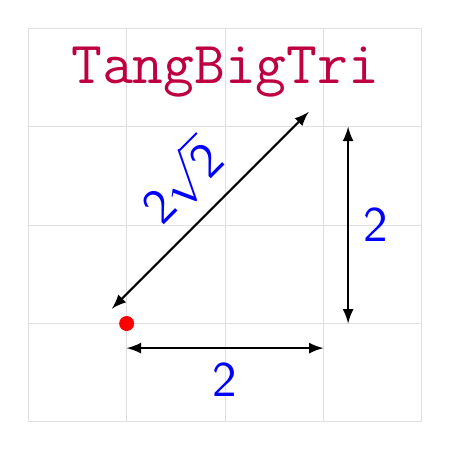
\begin{tikzpicture}[scale=1.25]
		\draw[thin,lightgray!50] (-1,-1) grid (3,3) ;
		\PieceTangram{TangBigTri} \filldraw[red] (0,0) circle[radius=2pt] ;
		\draw[thick,<->,>=latex] (0,-0.25)--(2,-0.25) node[blue,scale=1.5,midway,below,font=\large\sffamily] {2} ;
		\draw[thick,<->,>=latex] (2.25,0)--++(0,2) node[blue,scale=1.5,midway,right,font=\large\sffamily] {2} ;
		\draw[thick,<->,>=latex] (-0.15,0.15)--++(45:{sqrt(8)}) node[blue,scale=1.5,midway,sloped,above,font=\large\sffamily] {$\mathsf{2\sqrt{2}}$} ;
		\draw (1,3) node[scale=1.5,purple,below=1pt,font=\Large\ttfamily] {TangBigTri} ;
	\end{tikzpicture}
	~
	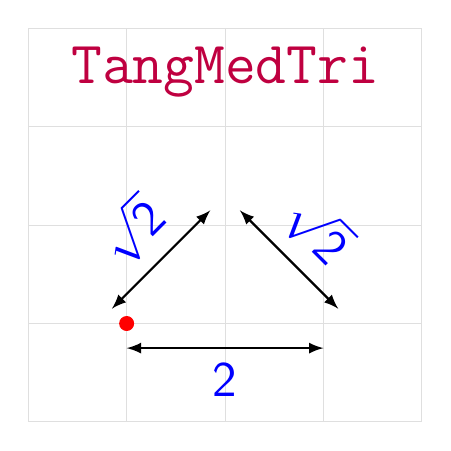
\begin{tikzpicture}[scale=1.25]
		\draw[thin,lightgray!50] (-1,-1) grid (3,3) ;
		\PieceTangram{TangMedTri} \filldraw[red] (0,0) circle[radius=2pt] ;
		\draw[thick,<->,>=latex] (0,-0.25)--(2,-0.25) node[blue,scale=1.5,midway,below,font=\large\sffamily] {2} ;
		\draw[thick,<->,>=latex] (-0.15,0.15)--++(45:{sqrt(2)}) node[blue,scale=1.5,midway,sloped,above,font=\large\sffamily] {$\mathsf{\sqrt{2}}$} ;
		\draw[thick,<->,>=latex] (2.15,0.15)--++(135:{sqrt(2)}) node[blue,scale=1.5,midway,sloped,above,font=\large\sffamily] {$\mathsf{\sqrt{2}}$} ;
		\draw (1,3) node[purple,scale=1.5,below=1pt,font=\Large\ttfamily] {TangMedTri} ;
	\end{tikzpicture}
	~
	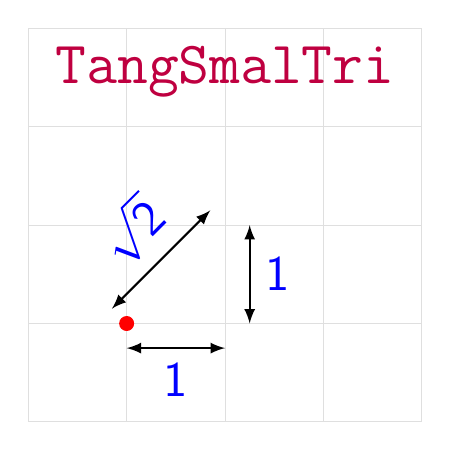
\begin{tikzpicture}[scale=1.25]
		\draw[thin,lightgray!50] (-1,-1) grid (3,3) ;
		\PieceTangram{TangSmalTri} \filldraw[red] (0,0) circle[radius=2pt] ;
		\draw[thick,<->,>=latex] (0,-0.25)--(1,-0.25) node[blue,scale=1.5,midway,below,font=\large\sffamily] {1} ;
		\draw[thick,<->,>=latex] (-0.15,0.15)--++(45:{sqrt(2)}) node[blue,scale=1.5,midway,sloped,above,font=\large\sffamily] {$\mathsf{\sqrt{2}}$} ;
		\draw[thick,<->,>=latex] (1.25,0)--++(0,1) node[blue,scale=1.5,midway,right,font=\large\sffamily] {1} ;
		\draw (1,3) node[purple,scale=1.5,below=1pt,font=\Large\ttfamily] {TangSmalTri} ;
	\end{tikzpicture}
	
	\smallskip
	
	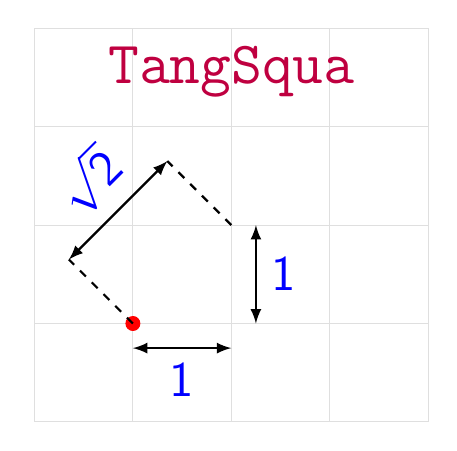
\begin{tikzpicture}[scale=1.25]
		\draw[thin,lightgray!50] (-1,-1) grid (3,3) ;
		\PieceTangram{TangSqua} \filldraw[red] (0,0) circle[radius=2pt] ;
		\draw[thick,<->,>=latex] (0,-0.25)--(1,-0.25) node[blue,scale=1.5,midway,below,font=\large\sffamily] {1} ;
		\draw[thick,<->,>=latex] (1.25,0)--++(0,1) node[blue,scale=1.5,midway,right,font=\large\sffamily] {1} ;
		\draw[thick,dashed] (0,0)--(-0.65,0.65) (1,1)--(0.35,1.65) ;
		\draw[thick,<->,>=latex] (-0.65,0.65)--++(45:{sqrt(2)}) node[blue,scale=1.5,midway,sloped,above,font=\large\sffamily] {$\mathsf{\sqrt{2}}$} ;
		\draw (1,3) node[purple,scale=1.5,below=1pt,font=\Large\ttfamily] {TangSqua} ;
	\end{tikzpicture}
	~
	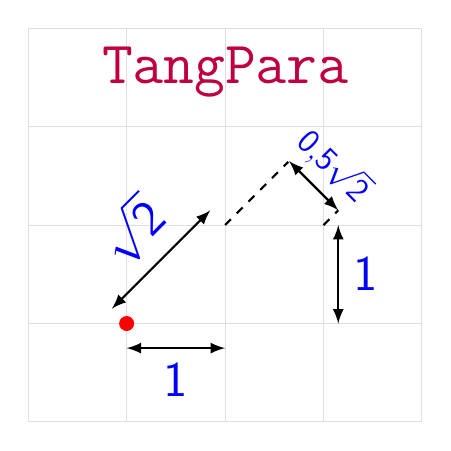
\begin{tikzpicture}[scale=1.25]
		\draw[thin,lightgray!50] (-1,-1) grid (3,3) ;
		\PieceTangram{TangPara} \filldraw[red] (0,0) circle[radius=2pt] ;
		\draw[thick,<->,>=latex] (0,-0.25)--(1,-0.25) node[blue,scale=1.5,midway,below,font=\large\sffamily] {1} ;
		\draw[thick,<->,>=latex] (-0.15,0.15)--++(45:{sqrt(2)}) node[blue,scale=1.5,midway,sloped,above,font=\large\sffamily] {$\mathsf{\sqrt{2}}$} ;
		\draw[thick,<->,>=latex] (2.15,0)--++(0,1) node[blue,scale=1.5,midway,right,font=\large\sffamily] {1} ;
		\draw[thick,<->,>=latex] (2.15,1.15)--++(135:{0.5*sqrt(2)}) node[blue,midway,sloped,above,font=\large\sffamily] {$\mathsf{0{,}5\sqrt{2}}$} ;
		\draw[thick,dashed] (2,1)--++(0.15,0.15) (1,1)--++(45:{0.5*sqrt(2)+0.2}) ;
		\draw (1,3) node[purple,scale=1.5,below=1pt,font=\Large\ttfamily] {TangPara} ;
	\end{tikzpicture}
\end{center}

Each \textit{piece} can :

\begin{itemize}
	\item rotated, thanks to \tikzlogo' option \texttt{rotate=...} ;
	\item fliped vertically or horizontally, thanks to \tikzlogo' option \texttt{xscale=-1} and \texttt{yscale=-1} ;
	\item moved, by placing it at point \texttt{(x,y)}.
\end{itemize}

Each piece comes with a \tikzlogo' style :

\begin{itemize}
	\item \texttt{TangPuzz} : piece of Tangram, \textit{full}, with a color (\Cle{black} by default) ;
	\item \texttt{TangSol} : piece of tangram, \textit{with white border}, with a color (\Cle{black} by default).
\end{itemize}

\pagebreak

\subsection{Positionning of the pieces}

A first methodis to use \texttt{pic} syntax in \tikzlogo{} :

\begin{PresentationCode}{listing only}
%environment or tikz command
\pic[style,rotate=...,xscale=...,yscale=...] at (x,y) {piece_name} ;
\end{PresentationCode}

The package \textsf{TangramTikz} proposes a specific command to place the pieces :

\begin{PresentationCode}{listing only}
%environment or tikz command
\PieceTangram[style={color}]<xscale=...,yscale=...,rotate=...>(x,y){piece_name}
\end{PresentationCode}

A Tangram is built form the 7 pieces, by :

\begin{itemize}
	\item \textit{putting} pieces at origin ;
	\item \textit{rotating/fliping} for the correct orientation ;
	\item \textit{translating} for the correct position.
\end{itemize}

\begin{PresentationCode}{}
%Correction colored version, initial size
\begin{EnvTangramTikz}
	\PieceTangram[TangSol={green}]({0},{0}){TangSqua}
	\PieceTangram[TangSol={red}]({-1.5},{1}){TangBigTri}
	\PieceTangram[TangSol={red}]<rotate=-90>({0.5},{3}){TangBigTri}
	\PieceTangram[TangSol={purple}]<xscale=-1,rotate=0>({2.5},{2}){TangPara}
	\PieceTangram[TangSol={blue}]({-1.5},{2}){TangSmalTri}
	\PieceTangram[TangSol={blue}]<xscale=-1,rotate=90>({-0.5},{2}){TangSmalTri}
	\PieceTangram[TangSol={orange}]({-0.5},{3}){TangMedTri}
	\filldraw[black] (0,0) circle[radius=2pt] ; %help
\end{EnvTangramTikz}
%Normal version, initial size
\begin{EnvTangramTikz}
	\PieceTangram[TangPuzz]({0},{0}){TangSqua}
	\PieceTangram[TangPuzz]({-1.5},{1}){TangBigTri}
	\PieceTangram[TangPuzz]<rotate=-90>({0.5},{3}){TangBigTri}
	\PieceTangram[TangPuzz]<xscale=-1,rotate=0>({2.5},{2}){TangPara}
	\PieceTangram[TangPuzz]({-1.5},{2}){TangSmalTri}
	\PieceTangram[TangPuzz]<xscale=-1,rotate=90>({-0.5},{2}){TangSmalTri}
	\PieceTangram[TangPuzz]({-0.5},{3}){TangMedTri}
\end{EnvTangramTikz}
\end{PresentationCode}

\pagebreak

\section{Automatic Method}

\subsection{Command}

Some predefined tangrams are present in the package \textsf{TangramTikz}, and thre's an independent \textsf{command} to "call" them :

\begin{PresentationCode}{listing only}
%independent command to display a Tangram
\TangramTikz[keys]<options tikz>{tangram_name}
\end{PresentationCode}

\begin{PresentationCode}{}
%independent command to display Cat/Boat/Kangaroo, with options by default
\TangramTikz{Cat}~~\TangramTikz{Boat}~~\TangramTikz{Kangaroo}
\end{PresentationCode}

\subsection{Keys, options and arguments}

The first argument, \textit{optional} and between \texttt{[...]}, give the keys :

\begin{itemize}
	\item the boolean \Cle{Puzzle} to display \textit{uni-}color pieces, without border ; \hfill~default : \Cle{true}
	\item the boolean \Cle{Correction} to display \textit{uni-}color pieces, with border ; \hfill~default : \Cle{false}
	\item \Cle{Color} to configure the \textit{uni-}color with the above bololeans ; \hfill~default : \Cle{black}
	\item the boolean \Cle{ColorCorrection} to display colored pieces with border ; \hfill~default : \Cle{false}
	\item \Cle{ColorList} which are the colors of the pieces (\texttt{BT,MT,ST,SQUA,PARA})  ;
	
	\hfill~default : \Cle{red,orange,blue,green,purple}
	\item \Cle{Sep}, the width of the border in \Cle{Correction} mode. \hfill~default : \Cle{1pt}
\end{itemize}

The second argument, \textit{optional} ans between \texttt{<...>}, give options to the \tikzlogo{} environnement, for example :

\begin{itemize}
	\item unit(s) change, scale change ;
	\item rotation, vertical alignment ;
	\item etc
\end{itemize}

The third argument, \textit{mandatory} and between \texttt{\{...\}} is the name of the predefined tangram :
%
\texttt{\begin{multicols}{5}
	\begin{itemize}
		\item Square
		\item Pinguin
		\item Boat
		\item Home
		\item FirTree
		\item Cat
		\item Swan
		\item Pyramid
		\item Duck
		\item Rocket
		\item Candle
		\item Shirt
		\item Fish
		\item Sailboat
		\item Kangaroo
		\item Dog
		\item Plane
		\item Rabbit
		\item Rooster
		\item Jogger
		\item Dancer
		\item Camel
	\end{itemize}
\end{multicols}}

\pagebreak

\begin{PresentationCode}{}
\TangramTikz{Rocket}~~
\TangramTikz[Color=red]{Rocket}~~
\TangramTikz[Correction]{Rocket}~~
\TangramTikz[Correction,Color=lightgray]{Rocket}~~
\TangramTikz[ColorCorrection,ColorList={orange,blue,yellow,green,pink},Sep=1mm]{Rocket}

\TangramTikz<scale=1.5,rotate=30>{Rocket}~~
\TangramTikz<scale=0.75,rotate=-90>{Rocket}
\end{PresentationCode}

\pagebreak

\part{Gallery of Tangrams}

\begin{PresentationCode}{}
\TangramTikz{Square}
\TangramTikz[Correction]{Square}
\TangramTikz[ColorCorrection]{Square}
\end{PresentationCode}

\begin{PresentationCode}{}
\TangramTikz{Pinguin}
\TangramTikz[Correction]{Pinguin}
\TangramTikz[ColorCorrection]{Pinguin}
\end{PresentationCode}

\begin{PresentationCode}{}
\TangramTikz{Boat}
\TangramTikz[Correction]{Boat}
\TangramTikz[ColorCorrection]{Boat}
\end{PresentationCode}

\begin{PresentationCode}{}
\TangramTikz{Home}
\TangramTikz[Correction]{Home}
\TangramTikz[ColorCorrection]{Home}
\end{PresentationCode}

\begin{PresentationCode}{}
\TangramTikz{FirTree}
\TangramTikz[Correction]{FirTree}
\TangramTikz[ColorCorrection]{FirTree}
\end{PresentationCode}

\begin{PresentationCode}{}
\TangramTikz{Cat}
\TangramTikz[Correction]{Cat}
\TangramTikz[ColorCorrection]{Cat}
\end{PresentationCode}

\begin{PresentationCode}{}
\TangramTikz{Swan}
\TangramTikz[Correction]{Swan}
\TangramTikz[ColorCorrection]{Swan}
\end{PresentationCode}

\begin{PresentationCode}{}
\TangramTikz{Pyramid}
\TangramTikz[Correction]{Pyramid}
\TangramTikz[ColorCorrection]{Pyramid}
\end{PresentationCode}

\begin{PresentationCode}{}
\TangramTikz{Duck}
\TangramTikz[Correction]{Duck}
\TangramTikz[ColorCorrection]{Duck}
\end{PresentationCode}

\begin{PresentationCode}{}
\TangramTikz{Rocket}
\TangramTikz[Correction]{Rocket}
\TangramTikz[ColorCorrection]{Rocket}
\end{PresentationCode}

\begin{PresentationCode}{}
\TangramTikz{Candle}
\TangramTikz[Correction]{Candle}
\TangramTikz[ColorCorrection]{Candle}
\end{PresentationCode}

\begin{PresentationCode}{}
\TangramTikz{Shirt}
\TangramTikz[Correction]{Shirt}
\TangramTikz[ColorCorrection]{Shirt}
\end{PresentationCode}

\begin{PresentationCode}{}
\TangramTikz{Fish}
\TangramTikz[Correction]{Fish}
\TangramTikz[ColorCorrection]{Fish}
\end{PresentationCode}

\begin{PresentationCode}{}
\TangramTikz{Sailboat}
\TangramTikz[Correction]{Sailboat}
\TangramTikz[ColorCorrection]{Sailboat}
\end{PresentationCode}

\begin{PresentationCode}{}
\TangramTikz{Kangaroo}
\TangramTikz[Correction]{Kangaroo}
\TangramTikz[ColorCorrection]{Kangaroo}
\end{PresentationCode}

\begin{PresentationCode}{}
\TangramTikz{Dog}
\TangramTikz[Correction]{Dog}
\TangramTikz[ColorCorrection]{Dog}
\end{PresentationCode}

\begin{PresentationCode}{}
\TangramTikz{Plane}
\TangramTikz[Correction]{Plane}
\TangramTikz[ColorCorrection]{Plane}
\end{PresentationCode}

\begin{PresentationCode}{}
\TangramTikz{Rabbit}
\TangramTikz[Correction]{Rabbit}
\TangramTikz[ColorCorrection]{Rabbit}
\end{PresentationCode}

\begin{PresentationCode}{}
\TangramTikz{Rooster}
\TangramTikz[Correction]{Rooster}
\TangramTikz[ColorCorrection]{Rooster}
\end{PresentationCode}

\begin{PresentationCode}{}
\TangramTikz{Jogger}
\TangramTikz[Correction]{Jogger}
\TangramTikz[ColorCorrection]{Jogger}
\end{PresentationCode}

\begin{PresentationCode}{}
\TangramTikz{Dancer}
\TangramTikz[Correction]{Dancer}
\TangramTikz[ColorCorrection]{Dancer}
\end{PresentationCode}

\begin{PresentationCode}{}
\TangramTikz{Camel}
\TangramTikz[Correction]{Camel}
\TangramTikz[ColorCorrection]{Camel}
\end{PresentationCode}

\newpage

\part{History}

\verb|v0.1.1|~:~~~~New models

\verb|v0.1.0|~:~~~~Initial version

\end{document}